\title{Aula 7 - Wired Equivalent Privacy (WEP)}

\author{Prof. Gabriel Rodrigues Caldas de Aquino}

\institute
{
    Instituto de Computação \\
    Universidade Federal do Rio de Janeiro\\
    gabrielaquino@ic.ufrj.br% Your institution for the title page
}
\date{Compilado em: \\ \today} % Date, can be changed to a custom date

%----------------------------------------------------------------------------------------
%    PRESENTATION SLIDES
%----------------------------------------------------------------------------------------



\begin{frame}
    % Print the title page as the first slide
    \titlepage
\end{frame}


\begin{frame}{Introdução ao WEP}
\begin{itemize}
    \item Nos primeiros cinco anos do padrão IEEE 802.11, apenas um método de segurança foi definido: o \textbf{Wired Equivalent Privacy (WEP)}.
    \item Muitas vezes, WEP foi identificado incorretamente como \textit{Wireless Effective Privacy} e outras variantes.
    \item Com o aumento da popularidade das redes Wi-Fi no ano 2000, a comunidade criptográfica começou a analisar o WEP e rapidamente encontrou vulnerabilidades.
    \item Já em 2001, ferramentas para quebrar o WEP em pouco tempo estavam disponíveis na Internet.
\end{itemize}
\end{frame}

\begin{frame}{Objetivos do WEP segundo o IEEE 802.11 (1999)}
\begin{itemize}
\item \textbf{Força Razoável}:
\begin{itemize}
    \item A segurança depende da dificuldade de descobrir a chave secreta por ataque de força bruta.  
    \item Relaciona-se ao tamanho da chave e à frequência de troca das chaves e do vetor de inicialização (IV).
\end{itemize}

\end{itemize}

\begin{itemize}
\item \textbf{Exportabilidade}:
\begin{itemize}
    \item Foi projetado de modo a facilitar a aprovação de exportação pelo Departamento de Comércio dos EUA.  
    \item No entanto, devido ao clima político e legal da época, não havia garantias de exportabilidade.
     \item O padrão IEEE 802.11 especificava apenas o uso de chaves de 40 bits.
    \item \textbf{Problema}: 40 bits é um tamanho muito pequeno para resistir a ataques de força bruta, \textbf{o que explicava sua aceitação nas regras de exportação}.
    \item \textbf{Exemplo de ideia da época}: Se um banco fosse utilizar LAN sem fio, teria seu próprio protocolo de segurança rodando sobre o WEP.
\end{itemize}

\end{itemize}


\end{frame}







\begin{frame}{Objetivos do WEP segundo o IEEE 802.11 (1999)}

\begin{itemize}
\item \textbf{Auto-Sincronização}:
\begin{itemize}
    \item O WEP é auto-sincronizável para cada mensagem
        \item Propriedade importante em algoritmos de enlace de dados, onde a perda de pacotes pode ser alta.

    \item Basicamente, isso significa que cada pacote deve ser encriptado separadamente, de forma que, dado um pacote e a chave, você tenha todas as informações necessárias para decriptá-lo.
    \item Claramente, não se deseja uma situação em que a perda de um único pacote torne todos os pacotes seguintes indecifráveis.
\end{itemize}
\end{itemize}

\begin{itemize}
\item \textbf{Eficiência}:
O algoritmo é eficiente, podendo ser implementado em \textbf{hardware ou software}.
\end{itemize}

\begin{itemize}
\item \textbf{Opcionalidade}:
A implementação e o uso do WEP eram \textbf{opcionais} no padrão IEEE 802.11.
\end{itemize}
\end{frame}

\begin{frame}{Como o WEP foi "vendido" na época}
\begin{itemize}
\item \textbf{Influência do Marketing}:
\begin{itemize}
    \item Na promoção do IEEE 802.11, a palavra "razoável" foi omitida 
    \item Na época WEP passou a ser descrito simplesmente como seguro.  
    \item Após a flexibilização das restrições de exportação, fabricantes criaram extensões não padronizadas com chaves de 104 bits
\item \textbf{Propaganda}:  WEP era "extremamente" ou "absolutamente" seguro.
\end{itemize}

\item \textbf{Efeito no Mercado}
Essas extensões de chave foram incorporadas à especificação Wi-Fi e se tornaram o padrão da indústria em 1999.  
Na visão dos gestores de marketing, o WEP estava agora completamente seguro.

    \item \textbf{IMPORTANTE: Erro na Definição de Segurança}:
    \begin{itemize}
        \item Aceitar o conceito de um nível "razoável" de segurança foi um erro.  
\item Só existem dois tipos de segurança: forte ou nenhuma.  
\item O padrão deveria: (i) OU ter incorporado uma solução realmente robusta OU deixado claro que a segurança deveria ser provida por outros meios (ex. VPN, HTTPS..).
    \end{itemize}
    

\end{itemize}
\end{frame}

\begin{frame}{Críticas ao WEP}
\begin{itemize}
    \item Alguns críticos acusam os projetistas do padrão IEEE 802.11 original por criarem o WEP com fraquezas inerentes.
    \item No entanto, é importante lembrar que, na época, o WEP \textbf{não foi projetado para prover segurança em nível militar}.
    \item O objetivo era fornecer uma proteção semelhante à de uma rede cabeada: \textbf{difícil, mas não impossível de quebrar}.
\end{itemize}
\end{frame}


\begin{frame}{Uso do WEP}
\begin{itemize}
    \item Para muitos usuários, o WEP foi a única escolha até a adoção de novos métodos de segurança no padrão IEEE 802.11.
    \item Mesmo com suas fraquezas, o WEP era considerado melhor do que não ter nenhuma proteção.
    \item O WEP cria uma \textbf{barreira mínima}, suficiente para desencorajar atacantes casuais, que preferem procurar redes totalmente abertas.
\end{itemize}

\begin{itemize}
\item \textbf{Eficácia do WEP em Ambientes Domésticos}:
\begin{itemize}
    \item A maioria dos ataques ao WEP depende da coleta de um número significativo de pacotes transmitidos.
    \item Em redes domésticas, onde o tráfego seria a ser pequeno, o WEP \textbf{poderia oferecer} um nível razoável de segurança.

\end{itemize}

\end{itemize}


\end{frame}



\begin{frame}{Funcionamento do WEP}
\begin{itemize}
    \item \textbf{Fases da segurança no WEP:}
    \begin{itemize}
        \item Autenticação: o dispositivo prova sua identidade ao ponto de acesso.
        \item Criptografia: garante a confidencialidade das mensagens após a autenticação.
    \end{itemize}
\end{itemize}
\begin{itemize}
    \item \textbf{Propósito da autenticação:}
    \begin{itemize}
        \item Permitir que cada parte prove que é quem afirma ser.
        \item Similar a assinar um cheque: confirma a identidade do remetente.
    \end{itemize}
\end{itemize}

\begin{itemize}
    \item \textbf{Proposito da criptografia}:
        \begin{itemize}
            \item Permitir que os dados trafegados não sejam vistos por quem está interceptando (Confidencialidade)
            \item Fazer com que quem envie ou receba dados na rede faça-o se possuir a chave.
        \end{itemize}
\end{itemize}

    
\end{frame}





\begin{frame}{Autenticação no WEP}
\begin{itemize}
    \item A autenticação WEP tem o objetivo de provar ao ponto de acesso legítimo que o dispositivo móvel conhece a chave secreta.
\end{itemize}

\centering
  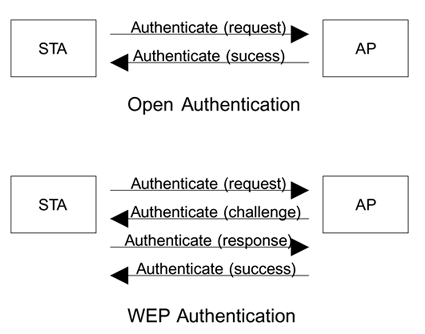
\includegraphics[width=0.55\linewidth]{Figuras/wep-auth.png}



\end{frame}




\begin{frame}{Formato da Mensagem de Autenticação (802.11)}
\begin{block}{Campos principais}
\begin{itemize}
    \item \textbf{Algorithm Number:} Indica o tipo de autenticação
    \begin{itemize}
        \item 0 – Open System
        \item 1 – Shared Key (WEP)
    \end{itemize}
    \item \textbf{Transaction Sequence:} Número da etapa na sequência de autenticação
    \begin{itemize}
        \item Mensagem 1, Mensagem 2, (e Mensagem 3 no caso do WEP)
    \end{itemize}
    \item \textbf{Status Code:} Indica sucesso ou falha na autenticação (última mensagem)
    \item \textbf{Challenge Text:} Usado apenas na autenticação por chave compartilhada (WEP)
\end{itemize}
\end{block}



\centering
  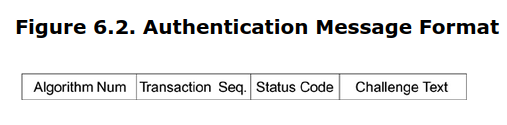
\includegraphics[width=0.55\linewidth]{Figuras/wep-authentication-message.png}



\end{frame}



\begin{frame}{Challenge-Response}
\begin{block}{Definição}
Processo de autenticação que verifica uma identidade exigindo que uma resposta correta seja fornecida a um \textbf{desafio} (\textit{challenge}).
\end{block}

\begin{block}{Como funciona em sistemas computacionais}
\begin{itemize}
    \item O sistema envia um valor imprevisível (desafio).
    \item O usuário deve calcular e enviar a resposta correta.
    \item A resposta é validada para confirmar a identidade.
\end{itemize}
\end{block}
\end{frame}


\begin{frame}{Autenticação WEP - Mecanismo de Challenge-Response}



\begin{itemize}
    \item Quando o dispositivo solicita autenticação, o ponto de acesso envia um número aleatório chamado \textbf{challenge text}.
    \begin{itemize}
        \item Um número arbitrário de 128 bits, preferencialmente aleatório.
    \end{itemize}
\end{itemize}



\begin{itemize}
    \item O dispositivo móvel então criptografa esse número com a chave secreta usando WEP e envia de volta ao ponto de acesso.
    \item Como o ponto de acesso lembra o número aleatório enviado, ele pode verificar se a resposta foi criptografada com a chave correta.
    \item O dispositivo deve conhecer a chave para criptografar o valor aleatório corretamente.
\end{itemize}



\end{frame}


\begin{frame}{Limitações da Autenticação no 802.11}

\begin{block}{Observações importantes:}
    \begin{itemize}
        \item Isso não prova ao dispositivo móvel que o ponto de acesso conhece a chave.
        \item Se um atacante estiver escutando, ele terá um par de \textit{plaintext-ciphertext} para começar ataques.
        \item Devido a essas vulnerabilidades, a Wi-Fi Alliance abandonou o uso desse mecanismo de autenticação.
    \end{itemize}
\end{block}

\begin{block}{Problemas}
\begin{itemize}
    \item O método de autenticação com WEP é praticamente inútil.  
    \item Na verdade, é pior que inútil, pois fornece ao atacante informações úteis para explorar.  
\end{itemize}
\end{block}


\end{frame}


\begin{frame}{WEP e o Processo de Autenticação}
\begin{itemize}
    \item Quando o WEP está habilitado, as mensagens de dados são criptografadas.  
    \item Objetivo: impedir que atacantes entendam o conteúdo mesmo escutando o tráfego.  
    \item O padrão IEEE 802.11 original previa duas fases:  
    \begin{enumerate}
        \item Autenticação.  
        \item Criptografia dos dados.  
    \end{enumerate}
    \item Para decodificar, é necessário conhecer a \textbf{chave secreta}.  
\end{itemize}
\end{frame}

\begin{frame}{RC4 no WEP}
\begin{itemize}
    \item O WEP utiliza a cifra de fluxo \textbf{RC4} (Schneier, 1996).  
    \item Funcionamento em alto nível:  
    \begin{itemize}
        \item Entrada: um byte do fluxo de dados por vez.  
        \item Saída: um byte diferente, aparentemente aleatório.  
        \item Resultado: a saída parece uma sequência de números aleatórios.  
    \end{itemize}
    \item A descriptografia é o processo inverso.  
    \item O mesmo segredo é usado tanto para criptografar quanto para descriptografar (cifra \textbf{simétrica}).  
\end{itemize}

\begin{figure}
    \centering
    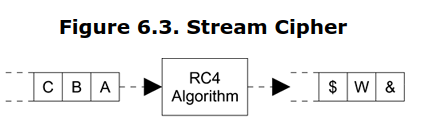
\includegraphics[width=0.55\linewidth]{Figuras/rc4-wep-stream.png}
    \caption{RC4 como cifra de fluxo no WEP}
\end{figure}
\end{frame}

\begin{frame}{RC4 e sua utilização no WEP}
    \begin{itemize}
        \item RC4 é simples de implementar, sem operações complexas como multiplicação.  
        \item Possui duas fases principais:
        \begin{itemize}
            \item \textbf{Inicialização}: tabelas internas são construídas a partir da chave.  
            \item \textbf{Encriptação}: os dados passam pelo algoritmo e são cifrados.  
        \end{itemize}
        \item \textbf{No WEP, ambas as fases ocorrem a cada pacote transmitido.}  
        \item Essa abordagem garante que a perda de um pacote não comprometa os seguintes.  
        \item Contudo, também introduz vulnerabilidades exploradas em ataques posteriores.  
        \begin{itemize}
            \item \textbf{Vocês podem imaginar quais seriam?}
        \end{itemize}
    \end{itemize}
\end{frame}


\begin{frame}{Problema de usar chave fixa no WEP}
    \begin{itemize}
        \item O WEP utiliza o algoritmo RC4.
        \item Com uma chave fixa: todos os pacotes seriam criptografados com a mesma chave.
        \item Consequência: textos repetidos geram sempre a mesma saída.
        \item Isso permite a um atacante identificar padrões, como endereços IP,
              já que certas partes dos pacotes se repetem.
    \end{itemize}

\begin{block}{Exemplo do Problema}
    \begin{itemize}
        \item Texto: \texttt{"Source Address"}
        \item Resultado cifrado (exemplo): \texttt{"b\%fP*aF\$!Y"}
        \item Sempre que o mesmo texto for cifrado com a mesma chave, o resultado será idêntico.
        \item Isso revela informação valiosa para o atacante.
    \end{itemize}
\end{block}
\end{frame}

\begin{frame}{Solução: Initialization Vector (IV)}
    \begin{itemize}
        \item Em vez de usar apenas a chave fixa, o WEP adiciona um número de 24 bits chamado \textbf{IV}.
        \item O IV muda a cada pacote transmitido.
        \item A chave efetiva passa a ser: \textbf{Chave Secreta (104 bits) + IV (24 bits)}.
        \item Isso garante que pacotes iguais gerem resultados diferentes.
    \end{itemize}

\begin{figure}
    \centering
    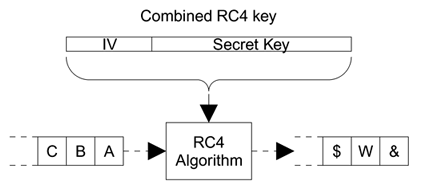
\includegraphics[width=0.55\linewidth]{Figuras/wep-iv-secret-key.png}
    \caption{RC4 com IV e Secret Key}
\end{figure}
\end{frame}

\begin{frame}{Limitação do IV}
    \begin{itemize}
        \item O IV é transmitido junto com o pacote, logo não é secreto.
        \item Chamar isso de “128-bit security” é enganoso, pois apenas 104 bits são realmente secretos.
        \item \textbf{Mesmo assim...} o uso do IV \textbf{dificulta} a identificação de padrões simples.
    \end{itemize}

\begin{figure}
    \centering
    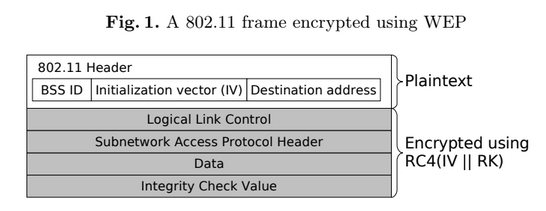
\includegraphics[width=0.9\linewidth]{Figuras/frame-encrypted-using-wep.png}

\end{figure}

\end{frame}

\begin{frame}{Problemas do Vetor de Inicialização (IV) no WEP}
    \begin{itemize}
        \item O IV não é secreto: é transmitido abertamente junto com os pacotes.  
        \item \textbf{O mesmo IV nunca deveria ser reutilizado com a mesma chave secreta}.  
        \item No WEP, o IV tem apenas \textbf{24 bits} $\Rightarrow$ cerca de 17 milhões de valores possíveis.  
        \item Em um ponto de acesso a 11 Mbps:
        \begin{itemize}
            \item todos os IVs podem ser usados em poucas horas.  
        \end{itemize}
        \item Reutilização de IVs é inevitável, pois as chaves raramente são trocadas.  
        \begin{block}{Problemas adicionais:}
            \begin{itemize}
            \item Muitos dispositivos reiniciam sempre com o mesmo IV (\textbf{Problema de implementação}).  
            \item Sequências “pseudoaleatórias” de IV podem se repetir em diferentes dispositivos.  
        \end{itemize}
        \end{block} 
        
        \item Consequência: IVs repetidos facilitam ataques contra o WEP.  
    \end{itemize}
\end{frame}

\begin{frame}{Funcionamento do WEP e Fragmentação}
    \begin{itemize}
        \item Aplicações enviam os dados.
        \item Os dados pode ser dividido em vários fragmentos.
        \item Cada fragmento é transformado em um \textbf{MPDU} (MAC Protocol Data Unit). 
        \item Para cada MPDU:
        \begin{itemize}
            \item É adicionado um cabeçalho MAC.
            \item É incluído um \textbf{ICV} no final.
            \item Cada fragmento é processado separadamente pelo WEP.
        \end{itemize}
        \item O processo de criptografia trata o MPDU como um bloco de bytes (10 a 1500 bytes).
        \item Antes da cifragem, adiciona-se o \textbf{Integrity Check Value (ICV)}.
    \end{itemize}
\end{frame}

\begin{frame}{Integrity Check Value (ICV)}
    \begin{itemize}
        \item Objetivo: detectar alterações nos dados durante a transmissão.
        \item Calculado como um CRC (Cyclic Redundancy Check) de 4 bytes.
        \item O ICV é adicionado \textbf{antes da criptografia} WEP.
        \item O CRC convencional ainda é adicionado \textbf{após a criptografia}.
        \item Ideia: como o ICV é cifrado, um atacante não poderia alterá-lo.
    \end{itemize}

\begin{block}{Limitações do ICV}
    \begin{itemize}
        \item Funciona contra \textbf{erros acidentais}, mas não contra ataques ativos.
        \item Atacantes podem recalcular o CRC após modificar a mensagem.
        \item Em teoria, o ICV deveria tornar a mensagem \textit{à prova de adulteração}.
        \item Na prática, há como contornar essa proteção.
    \end{itemize}
\end{block}
\end{frame}

\begin{frame}{Preparando o frame para transmissão}
    \begin{itemize}
    \item Pega os dados e calcula o ICV
        \item Após o ICV ser anexado, o quadro está pronto para criptografia.
        \item Seleciona-se um valor de \textbf{IV} (24 bits) e o anexa à chave WEP.
        \item O motor do \textbf{RC4} é inicializado.
        \item Cada byte do bloco (Dados + ICV) é processado $\rightarrow$ sai um byte criptografado.
        \item O quadro transmitido contém:
        \begin{itemize}
            \item IV (3 bytes) + KeyID (1 byte) no início.
            \item Dados criptografados + ICV criptografado.
            \item Cabeçalho MAC e CRC ao final.
        \end{itemize}
        \item Um bit no cabeçalho MAC indica que o quadro está protegido por WEP.
    \end{itemize}
\end{frame}

\begin{frame}{Recebendo o frame WEP}
    \begin{itemize}
        \item O receptor identifica o \textbf{bit WEP} no cabeçalho.
        \item Lê o valor do IV (3 bytes) e o KeyID (1 byte).
        \item Seleciona a chave WEP correta e inicializa o RC4.
        \item Processa cada byte do fluxo criptografado $\rightarrow$ obtém os dados originais.
        \item Como RC4 é simétrico, criptografia = decriptação (dupla aplicação anula o efeito).
        \item Calcula o ICV e compara com o recebido.
        \item Se válido, os dados são entregues para processamento superior.
    \end{itemize}
\end{frame}


\begin{frame}{Falhas do WEP - Autenticação}
    \begin{itemize}
        \item Autenticação serve para provar a identidade; idealmente, cada comunicação deve ser autenticada.
        \item Autenticação mútua é necessária em Wi-Fi:
        \begin{itemize}
            \item O usuário precisa verificar a rede.
            \item A rede precisa verificar o usuário.
        \end{itemize}
        \item Regras recomendadas para autenticação:
        \begin{enumerate}
            \item Método robusto que não possa ser falsificado.
            \item Identidade deve persistir em transações subsequentes e não ser transferível.
            \item Autenticação mútua.
            \item Chaves de autenticação devem ser independentes das chaves de criptografia.
        \end{enumerate}
    \end{itemize}
\end{frame}

\begin{frame}{Falhas na autenticação WEP}
\textbf{Mecanismo:}Challenge-response  \begin{itemize}

    \item 1. O AP envia uma string aleatória de números.  
    \item 2. A estação móvel cifra a string e envia de volta.  
    \item 3. O AP decifra e compara com a string original.  

\end{itemize}
\bigskip
\textbf{Problemas:}
\begin{itemize}
    \item \textbf{Regra 4 quebrada:} A chave usada na autenticação é a mesma usada para criptografia.
    \item \textbf{Regra 3 quebrada:} O AP não é autenticado; um AP malicioso pode enviar sucesso sem conhecer a chave.
    \item \textbf{Regra 2 quebrada:} Não há token para validar transações futuras.  
    \item \textbf{Regra 1 irrelevante:} Devido às falhas anteriores, a robustez da autenticação é comprometida.
\end{itemize}
\end{frame}


\begin{frame}{Ataque à autenticação WEP via XOR}
\textbf{Cenário:} Durante a autenticação, o AP envia um desafio de 128 bytes e a estação móvel responde cifrando com RC4.

\begin{columns}[t]
\column{0.55\textwidth}
\textbf{Transação capturada pelo atacante:}
\[
\text{Desafio (P)} \quad \rightarrow \quad \text{Texto claro}
\]
\[
\text{Resposta (C)} \quad \rightarrow \quad \text{Texto cifrado (RC4)}
\]

\column{0.45\textwidth}
\textbf{Extraindo o key stream:}
\[
R = C \oplus P
\]
\[
\text{Porque } P \oplus R = C \quad \text{e} \quad C \oplus P = R
\]
\end{columns}

\bigskip
\textbf{Consequência:}  
O atacante agora conhece o key stream \(R\) correspondente ao IV usado. Ele pode reutilizá-lo em futuras autenticações, conseguindo se autenticar sem conhecer a chave secreta.  

\textbf{Observação:} Essa falha fornece gratuitamente ao atacante os primeiros 128 bytes do key stream, que são os mais vulneráveis.
\end{frame}

\begin{frame}{Ataque à Autenticação por Challenge-Response}
\textbf{Contexto:} O mecanismo de autenticação do WEP usava um desafio (\textit{challenge}) que era criptografado pela estação e enviado de volta ao ponto de acesso.

\medskip
\textbf{Cenário:} Um atacante captura a seguinte troca de mensagens durante uma autenticação WEP:

\begin{itemize}
    \item Desafio (P) enviado pelo AP: \texttt{2A7F9C4E} (hexadecimal)
    \item Resposta (C) enviada pela estação: \texttt{D3B1AC8B} (hexadecimal)
\end{itemize}


\textbf{Pergunta:}
\begin{enumerate}


    \item Utilizando a operação XOR, calcule o keystream (R) usado pela estação para criptografar o desafio.

    \item Explique como um atacante, conhecendo este par (P, C), pode se autenticar fraudulentamente na rede no futuro, sem precisar conhecer a chave secreta WEP.
\end{enumerate}

\end{frame}


\begin{frame}{Cálculo do keystream (R) usando XOR}

\[
R = P \oplus C
\]

\[
R = \texttt{2A7F9C4E} \oplus \texttt{D3B1AC8B} = \texttt{F9CE30C5}
\]

2A7F9C4E =  0010.1010.0111.1111.1001.1100.0100.1110\\
D3B1AC8B= 1101.0011.1011.0001.1010.1100.1000.1011\\
--------------------------------------------------------------------------\\
F9CE30C5 = 1111.1001.1100.1110.0011.0000.1100.0101

\begin{block}{Atenção, para não confundir!}
    Esse R não é a chave secreta da rede WEP, mas sim o keystream (fluxo de chave) que o algoritmo RC4 gerou naquele momento específico, usando a combinação do Vetor de Inicialização (IV) e da chave secreta.
\end{block}
\end{frame}

\begin{frame}{Exploração pelo atacante}
    

\begin{itemize}
    \item O atacante agora conhece o \textbf{keystream} correspondente ao IV usado nesta autenticação.
    \item Ele pode reutilizar o keystream com o mesmo IV em futuras autenticações.
    \item Consequência: consegue se autenticar \textbf{sem precisar conhecer a chave secreta WEP}.
    \item Esse é o ponto inicial para ataques de quebra de WEP.

\end{itemize}
\end{frame}


\begin{frame}{Problema da persistência da autenticação no WEP}
\begin{itemize}




    \item A autenticação acontece apenas no início, durante o challenge-response.



    \item Depois disso, o sistema não emite nenhum tipo de “token” ou prova de identidade que o usuário possa apresentar nas transações subsequentes.

    \item Então, para todo o resto da comunicação, a rede não revalida a identidade do usuário, e tudo se baseia apenas na chave de criptografia usada para cifrar/decriptar os pacotes.
\end{itemize}    
\end{frame}

\begin{frame}{Replay Attack e WEP}
\textbf{Exemplo de ataque:}
\begin{itemize}
    \item Um invasor captura quadros (frames) entre um AP e um dispositivo móvel usando um sniffer.
    \item Observa mensagens criptografadas e seu tamanho, sem decifrar o conteúdo.
    \item Quando a usuária legítima se desconecta, o invasor se conecta usando o MAC da vítima.
    \item O invasor reenvia (replay) uma mensagem previamente capturada.
    \item O AP aceita a mensagem, passando-a ao servidor, que autentica o invasor sem perceber a fraude.
\end{itemize}

\bigskip
\textbf{Problema:}
\begin{itemize}
    \item WEP não possui proteção contra replay.
    \item Sequência de número no MAC não é protegida pelo WEP.
    \item Mensagens antigas podem ser reenviadas sem precisar quebrar a criptografia.
    \item Consequência: invasor consegue se autenticar indevidamente.
\end{itemize}
\end{frame}

\begin{frame}{Falha do WEP na Detecção de Modificação de Mensagens}
\textbf{Objetivo do WEP:} prevenir alterações nos dados transmitidos usando o \textit{Integrity Check Value (ICV)}.

\medskip
\textbf{Como funciona:}
\begin{itemize}
    \item O ICV é um valor CRC de 32 bits calculado sobre os dados.
    \item ICV é adicionado ao final da mensagem e toda a sequência é criptografada.
    \item Teoricamente, alterações no ciphertext seriam detectadas na decriptação.
\end{itemize}

\medskip
\textbf{Problema:}
\begin{itemize}
    \item O CRC é linear: é possível prever como o ICV muda ao alterar bits da mensagem.
    \item A operação XOR usada na criptografia permite \textit{bit flipping}: alterar bits no ciphertext altera os mesmos bits na mensagem decifrada.
    \item Um atacante que conheça os bits certos pode modificar a mensagem e ajustar o ICV correspondente, mantendo a integridade aparente.
\end{itemize}

\medskip
\textbf{Conclusão:} WEP não fornece proteção efetiva contra modificações no ciphertext.
\end{frame}

\begin{frame}{Por que o IV é importante no WEP?}
\textbf{Função do IV (Initialization Vector):}  
\begin{itemize}
    \item Adicionado à chave secreta para formar a chave de criptografia usada pelo RC4.
    \item Garante que duas mensagens idênticas não gerem o mesmo ciphertext.
\end{itemize}

\medskip
\textbf{E se não houvesse IV?}  
\begin{itemize}
    \item RC4 seria inicializado sempre no mesmo estado.
    \item O fluxo de chave (key stream) seria idêntico para todos os frames.
    \item Consequência: um atacante que descubra o fluxo de chave de um frame pode descriptografar todos os outros frames.
    \item Não seria necessário conhecer a chave secreta!
\end{itemize}
\end{frame}

\begin{frame}{IV diferente para cada frame}
\textbf{Por que usar IV diferente em cada frame?}
\begin{itemize}
    \item Adicionando o IV à chave secreta, o RC4 é inicializado em um estado diferente a cada frame.
    \item Consequência: o fluxo de chave (\emph{key stream}) é diferente para cada criptografia.
\end{itemize}

\medskip
\textbf{IV constante ou reutilizado é problemático:}
\begin{itemize}
    \item IV constante $\rightarrow$ mesmo problema do caso de chave fixa.
    \item IV reutilizado $\rightarrow$ permite que atacantes detectem padrões e quebrem a criptografia.
    \item Reuso inevitável se o número de IVs possíveis é limitado (24 bits no WEP).
    \item Seleção aleatória de IVs aumenta o risco de repetição cedo (paradoxo do aniversário).
\end{itemize}
\end{frame}

\begin{frame}{Paradoxo do Aniversário e IVs no WEP}
\textbf{Paradoxo do Aniversário:}
\begin{itemize}
    \item Probabilidade de pelo menos duas pessoas compartilharem o mesmo aniversário.
    \item Surpreendentemente, com apenas 23 pessoas, a probabilidade $>$ 50\%.
    \item Explicação: existem $23 \times 22 / 2 = 253$ pares possíveis.
\end{itemize}

\medskip
\textbf{Aplicação em criptografia:}
\begin{itemize}
    \item Ataques de colisão (\emph{birthday attack}) em funções hash.
    \item Similarmente, reuso de IVs em WEP aumenta a chance de colisões no fluxo de chave.
\end{itemize}

\medskip
\textbf{Lição para WEP:} O número limitado de IVs (24 bits) faz com que colisões aconteçam cedo, tornando o sistema vulnerável.
\end{frame}

\begin{frame}{Reuso de IVs no WEP}
\textbf{Problema:} IVs de 24 bits são limitados e podem se repetir rapidamente.  

\medskip
\textbf{Solução ideal:} incrementar o IV a cada quadro enviado para maximizar o tempo até uma repetição.  

\medskip
\textbf{Exemplo prático:}
\begin{itemize}
    \item IV de 24 bits $\rightarrow$ 16.777.216 valores possíveis.
    \item IEEE 802.11b transmite ~500 quadros/s.
    \item Espaço de IVs esgotado em cerca de 7 horas.
\end{itemize}

\medskip
\textbf{Problemas reais:}
\begin{itemize}
    \item Vários dispositivos usando o mesmo IV/ chave $\rightarrow$ colisões mais cedo.
    \item Erros de implementação: alguns fabricantes reiniciam o IV em 0 após reinício.
    \item Resultado: repetição de IV é comum e vulnerabilidade explorável.
\end{itemize}
\end{frame}
